Eine große Herausforderung bei der Modellierung des Softwareentwicklungsprozesses war eine genaue Momentaufnahme eines kontinierlichen arbeitenden Prozesses. 

\begin{figure}[p]
    \centering
    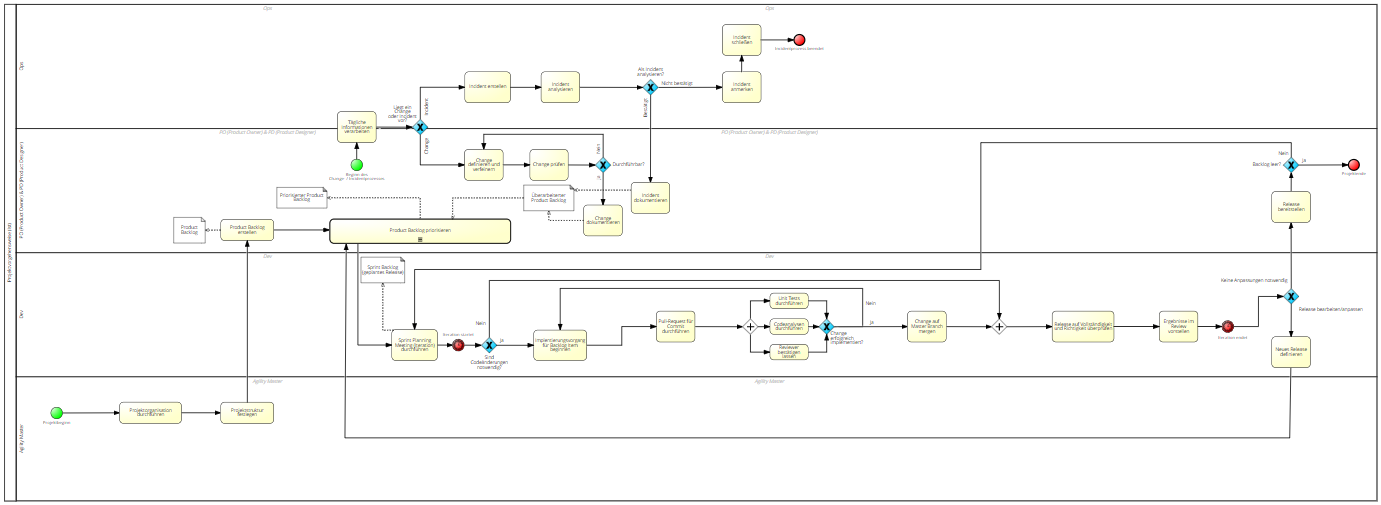
\includegraphics[angle=90, scale=0.7]{Bilder/IST-Prozess.png}
    \caption{Softwareentwicklungsprozess im IST-Zustand basierend auf dem HAF-Projekt}
\end{figure}

Da das DevOps-Team mit agilen Methoden wie Scrum und Kanban arbeitet, erwies sich die Modellierung des IST-Prozesses basierend auf einem Sprint am geeignesten. 
\dwi{.."DevOps-Team mit agilen Methoden wie Scrum und Kanban arbeitet" .. hier beschreibst du den IST-prozess. welchen genau? einen generischen? einen exemplarischen? das sollte klar herauskommen, das du in diesem kapitel (deiner arbeit) den prozess aus einem konkreten devops-projekt betrachtest.}

Der Prozess wurde \dwi{schreibst du präsens oder vergangenheit? das muss 100\% konsistent sein. ich empfehle überall präsens, weil es die faktenlage zeitlich neutral beschreibt.} zunächst in vier essentielle Rollen unterteilt, die bei der Softwareentwicklung als DevOps-Team beteiligt sind: 

\paragraph{Agility Master}

Der Agility Master verantwortet einen effektiven und effizienten Prozess und stellt sicher, dass die Regeln des agil und Lean Management eingehalten werden. 

Ferner fungiert der Agility Master als ein Moderator für Team-Ereignisse und versucht Probleme und Hindernisse zeitnah zu lösen. 

Der Agility Master ist mit dem Scrum Master identisch. \dwi{warum führst du dann den namen agility master ein? es hilft dem leser (der nicht aus HAF kommt) nicht, hier einen begriff zu lesen der dann am ende mit einem konzept verglichen wird, das er schon kennt.}

\paragraph{Dev}

Diese Rolle entspricht der Rolle des Softwareentwickler oder Development-Teams. 

Je nach Projektanforderungen kann sich die Rolle des Entwicklers beispielsweise auf das Frontend- oder Backendentwicklung richten.

\paragraph{Product Owner und Product Designer}
\dwi{Product Designer ist eine kreation in unserem projekt, und würde in der scrum-welt eher als proxy-po bezeichnet werden. in deinem kontext hilft es aber beides nicht um deine inhalte zu transportieren - nimm nur PO und gut.}

Zunächst fungiert der Product Owner als die Schnittstelle zwischen verschiedenen Stakeholdern oder Kunden und dem Entwicklungsteam. 

Er vertritt demnach die Interessen des Kunden in den Entwicklungsprozess, ohne aktiv in die Softwareentwicklung einzugreifen.

Ferner erstellt der Product Owner den Product Backlog und legt die Reihenfolge der Items, die bearbeitet werden müssen, fest. 

Wie der Name schon sagt, beschreibt die Rolle des Product Designers die Gestaltung oder den Entwurf des Produkts. 

Hierzu gehören die Definitionen von UX-Anforderungen und Spezifikationen oder die Schaffung von Schnittstellen, im Hinblick auf die Fuktionalität und das erwartende Verhalten des Produkts. 

Innerhalb des HAF-Teams überschneiden sich die Rollen des Product Owner und des Product Designers, weshalb diese beiden Positionen in einer Swimlane dargestellt werden.  

\paragraph{Ops}
\dwi{du hast jetzt zum einen konkrete rollen die an personen hängen als swimlanes, und dann zwei lanes die an "dev" und "ops" hängen - das sind logische tätigkeitsbereiche. das ist "ungenau". entscheid dich für eine konsistente unterteilung.. und "dev" und "ops" zu trennen ist eigentlich nochmal eine ganz eigene diskussion. vllt kannst die beiden lanes auch zusammenführen unter "developer", sofern du beim rollenbasierten schnitt bleibst.}

Die Rolle des Administratoren oder IT-Betrieb entspricht dem anderen Teil des DevOps-Teams. 

In erster Linie sorgt diese Rolle für die Stabilität der IT-Infrastruktur und ermöglichen einen durchgängigen, laufenden Betrieb.  

\begin{figure}[h]
    \centering
    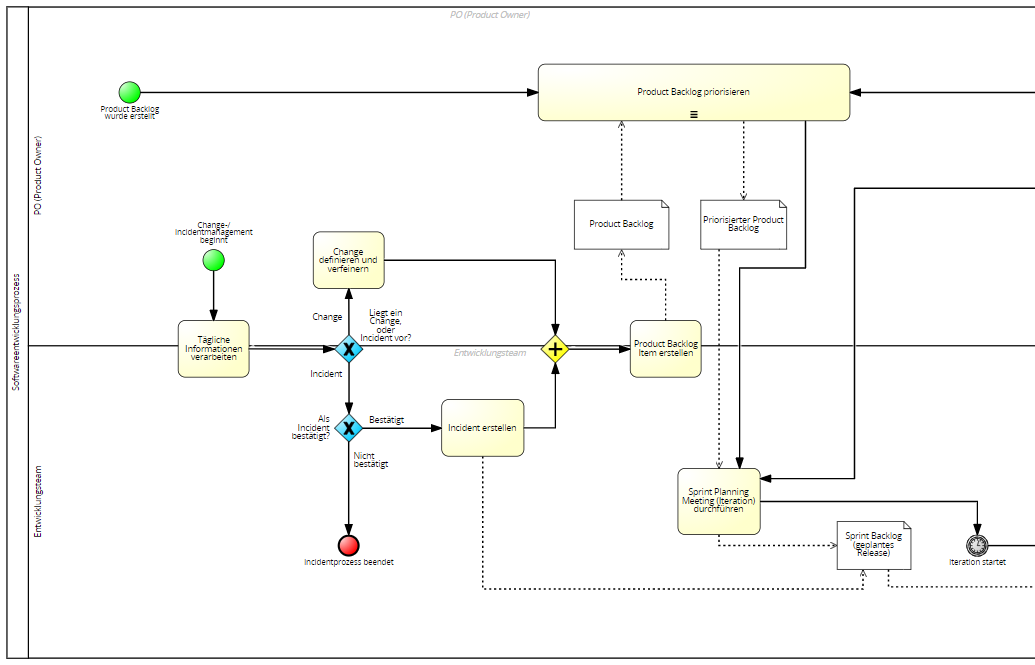
\includegraphics[scale=0.7]{Bilder/IST-Prozess_first Part.png}
    \caption{Erster Teil des Softwareentwicklungsprozess im IST-Zustand basierend auf dem HAF-Projekt}
\end{figure}

\newpage Startpunkt des Prozesses liegt beim Agility Master, indem die Projektorganisation zunächst durchgeführt und die Projektstruktur festgelegt wird.
\dwi{wenn du hier die schritte so genau erklärst, wäre eine visuelle nummerierung in der grafik und in den schritten vielleicht angebracht. oder du lässt das detailgrad weg und beschreibst nur den engeren kontext genauer.}

Zu beachten ist, dass diese zwei Aufgaben ausschließlich am Anfang eines jeden Projekts und nicht in laufenden Projekten stattfinden. 

Nachdem das Product Backlog erstellt wurde muss dieses vom Product Owner priorisiert werden. 

Die Priorisierung findet sequentiell statt, da mehrere Entwicklungen und Änderungen eines Items des Product Backlogs parallel und gleichzeitig und nicht als eine Aufgabenschleife stattfinden. 

Diese Änderungen fließen in den priorisierten Backlog ein. 

Ist die Priorisierung erfolgt, startet die Iteration mit dem Sprint Planning Meeting. 

Abhängig von den verfügbaren Kapazitäten und den Ergebnissen des letzten Sprints wird entschieden, welche User Stories zuerst bearbeitet werden. 

Die ausgewählten User Stories bilden den Sprint Backlog. 

Parallel zu den täglichen Entwicklungen beginnt der Change-/Incidentprozess, bei dem zunächst die täglichen Informationen verarbeitet werden. 

Der Changeprozess bescheibt den prozess für eine Änderung, die sich auf eine geplante Modifikation der Definition eines bestehenden oder neuen Produkts bezieht und für die das DevOps-Teams verantwortlich ist. 

Der Prozess umfasst die Erfassung jedes Requests, die Dokumentation, Genehmigung und Kontrolle und stellt sicher, dass Change Requests definiert, geplant, effizient, wirtschaftlich und mit vertretbarem Risiko abgewickelt werden. 

Ein Ziel des Change Managements ist es, die Nachvollziehbarkeit von Anforderungen und Änderungen zu gewährleisten.

Incident Management umfasst den gesamten organisatorischen und technischen Prozess für Reaktionen und Maßnahmen auf Störungen des IT-Betriebs.

Das Spektrum möglicher Incidents reicht von Fehlermeldungen durch Anwender bis hin zu automatisierten Alarmen und Warnungen durch das Monitoring.

Das Ziel des Incident Managements ist die Wiederherstellung eines zugesagten Dienstes in einem definierten Prozess und in optimaler Zeit. 

Dies kann auch Umgehungslösungen beinhalten. 

Incident Management deckt keine (neuen) Anforderungen, Wünsche, Anfragen oder ähnliches ab.  

Obwohl der Change- und Incidentprozess vom Product Owner bzw. Designer begonnen wird, ist dieser ausschließlich für den Changeprozess verantwortlich. 

Der Incidentprozess wird anhand des täglichen Monitorings vom Ops-Verantwortlichen durchgeführt. 

Nach der Verarbeitung der täglichen Informationen, werden die auftretenden Bugs zunächst in Incident und Changeprozesses unterschieden, da beide Prozesse werden unterschiedlich behandelt werden.

Innerhalb des Changeprozesses werden die Änderungen definiert und verfeinert. 

Nachdem die Änderung geprüft wurde, muss entschieden werden, ob die Änderung durchführbar also entwickelt werden kann. 

Ist dies der Fall wird die Änderung dokumentiert und fließt in den überarbeiteten Product Backlog ein, bei dem die Items wiederrum innerhalb des Product Backlogs priorisiert werden. 

Sollte der Change nicht durchzuführen sein, müssen die Definitionen und Verfeinerungen angepasst werden.

Innerhalb des Incidentprozesses wird der Incident zunächst erstellt und analysiert.

Sollte der Bug als Incident bestätigt werden, so wird dieser dokumentiert und fließt in das überarbeitete Product Backlog und wiederrum in das priorisierte Product Backlog ein. 

Falls dies nicht der Fall ist, wird der Incident angemerkt und geschlossen, wodurch der Incidentprozess ab diesem Zeitpunkt geschlossen wird. 

\begin{figure}[h]
    \centering
    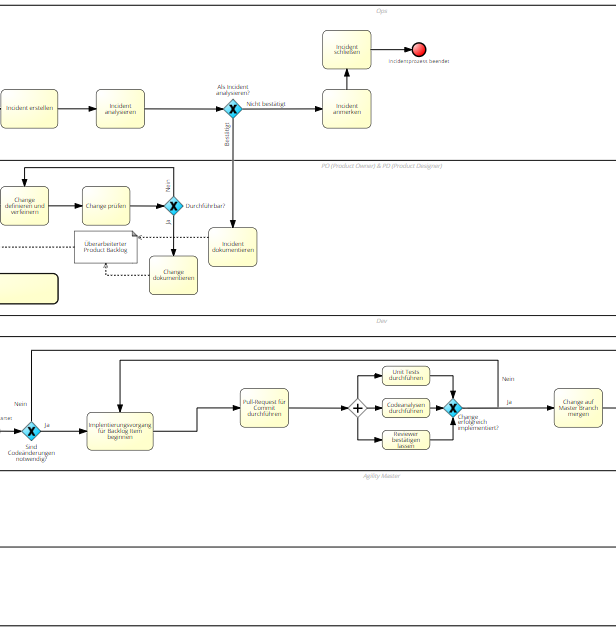
\includegraphics[scale=0.8]{Bilder/IST-Prozess_second Part.png}
    \caption{Zweiter Teil des Softwareentwicklungsprozess im IST-Zustand basierend auf dem HAF-Projekt}
\end{figure}

Sobald die Iteration startet, muss zunächst überprüft werden, ob Codeänderungen notwendig sind. 

Dies kann sich auf Änderungen eines vorhandenen Codes oder auf eine Neuimplementierung beziehen. 

Sobald keine Änderungen notwendig sind, bleibt das entsprechende Item im priorisierten Product Backlog und wird im Release auf seine Vollständigkeit und Richtigkeit überprüft.

Nachdem der Pull-Request für das Commit durchgeführt wurde, werden mehrere Aufgaben parallel erledigt. 

Dazu gehört die Durchführung der Unit-Test und Codeanalyse und die Bestätigung des Reviewer.

Sobald alle Änderungen erfolgreich implementiert worden sind, werden diese auf das Master Branch gemergt. 

\begin{figure}[h]
    \centering
    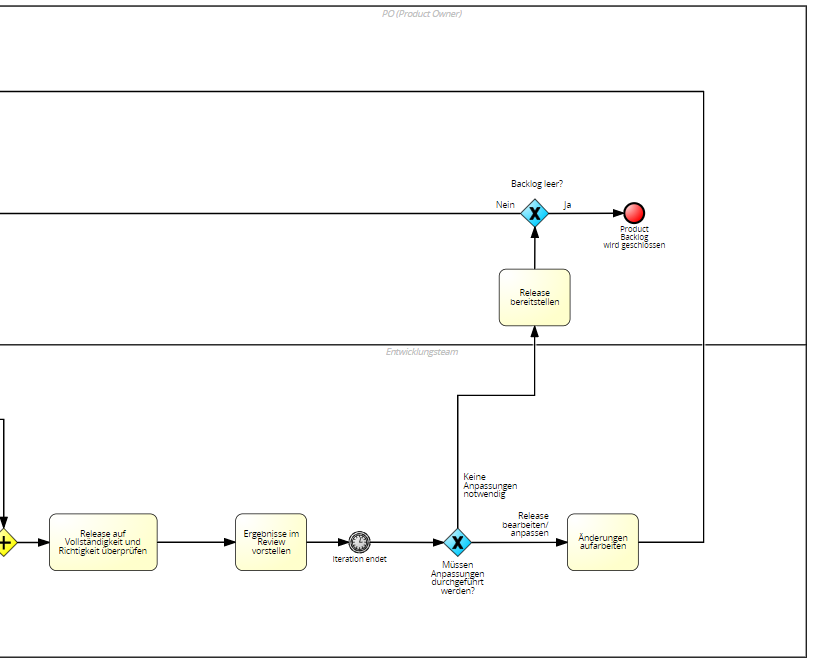
\includegraphics[scale=0.8]{Bilder/IST-Prozess_third Part.png}
    \caption{Dritter Teil des Softwareentwicklungsprozess im IST-Zustand basierend auf dem HAF-Projekt}
\end{figure}

Nachdem das Release auf seine Vollständigkeit und Richitgkeit überprüft worden ist, wird dieses im Review vorgestellt. 

Ab diesem Zeitpunkt endet die Iteration. 

Werden weitere Anpassungen benötigt, muss das neue Release bearbeitet und definiert werden, wobei diese in das priorisierte Backlog zurückfließen.

Sind keine Änderungen notwendig, wird das Release bereitgestellt. 

Das Projekt endet sobald das product Backlog leer ist.


%Frage an Daniel: Soll ich die BPMN-Modellierung kurz erläutern? 
%Eigentlich finde ich das nicht sinnvoll, weil der Prof. sich top in BPMN auskennt
%Aber vllt fürs Verständnis???? Wenn nicht im text, dann im Anhang ???















